\documentclass[journal]{IEEEtran}
\usepackage[spanish]{babel}
\usepackage[utf8]{inputenc}
\usepackage{graphicx}
\graphicspath{ {images/} }
%\usepackage{enumerate}
\usepackage{amsmath}
\usepackage{mathtools}
\usepackage{float}
\usepackage{amssymb}
\usepackage{listings}
\usepackage{hyperref}
%\usepackage{caption}
\usepackage[justification=centering]{caption}
\usepackage[font=scriptsize,labelfont=bf]{caption}
\renewcommand{\IEEEkeywordsname}{Palabras clave}
%\renewcommand{\table}{TABLA}
\renewcommand\spanishtablename{Tabla}
\renewcommand\lstlistingname{Salida}

\bgroup
\def\arraystretch{1.5}

\hypersetup{
    colorlinks=true,
    linkcolor=black,
    filecolor=magenta,      
    urlcolor=blue,
}


\lstset{
basicstyle=\footnotesize
%,
%numbers=left
}

\begin{document}

\title{\textbf{Laboratorio 1: Potencia \\ en aplicaciones domésticas}}
\author{
  \IEEEauthorblockN{ Jorge Lambra\~no$^3$, Julian Rojas$^2$, 
  Juan Sánchez$^3$\vspace{0.2cm}}\\
  \IEEEauthorblockA{\texttt{\small{$^1$jelambrano, $^2$drojasj,
   $^3$paradac @uninorte.edu.co
   }}}
}

\markboth{Laboratorio 1: Potencia en aplicaciones 
domésticas}%
{Shell \MakeLowercase{\textit{et al.}}: Bare Demo of IEEEtran.cls 
for Journals}
	
\maketitle

\begin{abstract}
This report presents the design and implementation 
of a security box and a dimmer circuit using DIACs 
and TRIACs. The reader also can find  the validation 
review with the theoretical model seen in class.    
\end{abstract}

%-----------------------------------------------------------

\begin{IEEEkeywords}  
%Current, Power, Power Factor, Voltage, Waveform.
Armónico, Corriente, Distorsión, Factor de Potencia,  Potencia, Tensión, Transformada de Fourier, Voltaje. 
\end{IEEEkeywords}

%-----------------------------------------------------------
\IEEEpeerreviewmaketitle
%--------------------------------------------------------------------------

\section{INTRODUCCIÓN}

El objetivo principal de esta práctica es realizar 
un análisis de la forma de onda y las mediciones 
de tres tipos diferentes de carga. Dentro de la caja 
de seguridad hay un fusible para proteger el equipo 
de cualquier corto circuito. Usamos una resistencia 
de 1 $\Omega$ y 10 W para medir la corriente dividiendo 
la tensión entre 1 para obtener el valor actual. 
Todos los dispositivos electrónicos están compuestos 
de resistencias, condensadores e inductancias, un 
soldador es una carga lineal resistiva, requieren calor 
para funcionar. El voltaje medido sería el mismo que 
el de la fuente, pero la corriente variará según el 
consumo de energía del dispositivo. Esperamos la misma 
forma de onda para el voltaje y la corriente y ningún 
cambio de fase entre ellos.\\

Un taladro es una carga lineal inductiva, basado 
en el hecho de que los motores están hechos de 
bobinas. Debería haber un cambio de fase entre el 
voltaje y la corriente. La computadora portátil 
es una carga no lineal, la forma de onda del voltaje 
sería la misma, pero esperamos una forma diferente 
para la corriente. \\

La segunda parte consiste en diseñar y desarrollar 
un controlador de CA compuesto por un DIAC y un 
QUADRAC. Este tipo de circuito puede cambiar el 
voltaje RMS en los terminales de una carga lineal 
manipulando el ángulo de disparo del QUADRAC usando 
un potenciómetro. La carga ya no será lineal debido 
al circuito resultante entre la bombilla y el 
controlador AC.


%--------------------------------------------------------------------

\section{PROCEDIMIENTO Y ANÁLISIS DE RESULTADOS}

\subsection{Cálculos de Potencia}

El objetivo de esta práctica es medir el consumo eléctrico 
de dispositivos cotidianos, tales como computadores 
portátiles, un pequeño taladro y un cautil. Teniendo en 
cuenta los valores altos de tensión y corriente que se 
pueden encontrar en instalaciones eléctricas domésticas, se
tomaron todas las precausiones necesarias para garantizar 
seguridad a los dispositivos, instrumentos de medición y 
a las personas que realizan la medición. Para poder 
obtener los valores de tensión, corriente y corriente se 
diseñó un circuito que junto con el osciloscopio, es capaz de
permite la obtención de valores de tensión y corriente. El 
diseño del circuito se encuentra ilustrado en la Figura 
\ref{circuit_diagram}. \\

%The purpose of this practice is to measure the 
%power consumption on electrical home devices, such 
%as a laptop, a drill and a soldering iron. Taking into 
%account that they work with high values of voltage 
%and current compared with previous labs, precautions 
%were taken in order to protect the devices and our 
%integrity. The Figure \ref{circuit_diagram} 
%shows the circuit proposed by the teacher to measure 
%voltage and current safely. 

\begin{figure}[h]
\centering
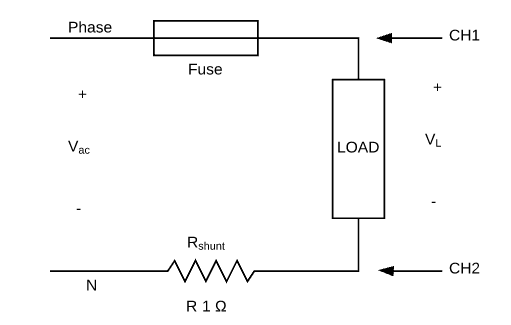
\includegraphics[clip,width=0.9\columnwidth]{circuit_diagram.png}
\caption{Circuito utilizado para la obtención \\
de los valores de corriente y tensión.}
\label{circuit_diagram}
\end{figure}

\textit{CH1} y \textit{CH2} representan los puntos donde
se toman el osciloscopio toma las medidas a través de las 
sondas de los canales 1 y 2 del osciloscopio,
\textit{Phase} y \textit{N} corresponden a la fase y 
al neutro de la red a la que se conecta el circuito. 
\textit{V\textsubscript{ac}} representa 
la onda de 120V\textsubscript{rms} 
que entrega la red eléctrica. 
\textit{Fuse} representa un fusible cuyo valor se explicará 
más adelante, \textit{Rshunt} representa una resistencia 
de potencia de 1 $\Omega$ y 10 W. \textit{LOAD} corresponde
al dispositivo al que se va a realizar la
medición.\\ 

Se puede observar del
gráfico que el valor de tensión que cae en el dispositivo
es la diferencia de los datos que se obtienen en los canales 
del osciloscopio. $V_L = CH1 - CH2$. Y la corriente que 
pasa a través del dispositivo es la razón entre la tensión 
que se obtiene en el canal \textit{CH2} y el valor de la 
resistencia. Esto es el valor del canal, puesto que 
la resistencia es de 1 $\Omega$. Esta información es muy
últil para los cálculos de potencia que se explicarán más 
adelante.\\

%obtained from the university phase line, \textit{Fuse}
%represents a 3A circuit breaker, \textit{Load} represents 
%the load and \textit{Rshunt} 
%represents the 1 $\Omega$ and 10 W 
%power resistor. We chose a small value for the resistor 
%to do not affect the functioning of the circuit. \\

%The gauge of the wire was selected depending on maximum 
%current needed by the higher power load according to 
%electrical parameters 
%of each device. Current values of devices are 
%shown on the Table \ref{current_table}. Based on this, 
%AWG 14 wire was selected to build the power meter, because 
%it is able to conduct a maximum of 15 A\textsubscript{rms}.
%In addition to this, the circuit uses a 3A fuse to protect
%load and wires of high currents.\\

\begin{table}[h]
\centering
\begin{tabular}{|l|p{1.2cm}|p{1.5cm}|p{1.5cm}|}
\hline 
Dispositivo & Potencia (W) & Tensión (V\textsubscript{rms}) 
& Corriente (A\textsubscript{rms}) \\ \hline 
Cautil 	&  40	& 120 	& 0.33 \\ \hline 
Taladro 		& 130	& 120   & 1.08 \\ \hline 
Portátil 		& 140 	& 120   & 1.16 \\ \hline 
Bombillo		& 70  	& 120   & 0.58 \\ \hline 
Resistencia & 10 & - & 3.17 \\ \hline
\end{tabular}
\caption{Power and current values of each device.}
\label{current_table}
\end{table}

Con respecto al calibre del alambre, fue seleccionado 
dependiendo de la máxima corriente que necesita cada 
dispoitivo, de acuerdo con los parámetros eléctricos 
que se muestran en la descripción del dispositivo. Estos
valores de corriente son mostrados en la Tabla
\ref{current_table}. Basándose en la 
Tabla \ref{current_table} se seleccionó un alambre 
AWG 14 capaz de soportar una corriente máxma de 
15A\textsubscript{rms}, puesto que es que utiliza 
normalmente en instalaciones eléctricas domésticas. 
La corriente máxima que sorporta el fusible es 
3A\textsubscript{rms}, se escogió este valor basándose
en la máxima corriente que es capaz de soportar la 
resistencia. \\

El circuito se introdujo dentro de una caja 4x4, el 
fusible se ubicó de tal forma que no fuese necesario 
abrir la caja en caso que fuera necesario reemplazarlo. 
Además se colocaron 
cuatro borneras para poder medir de forma más segura 
usando las sondas del osciloscopio. \\

%The circuit is inside a 4x4 box with a fuse holder to 
%change the breaker, 4 measuring terminals; the white 
%one for neutral, green one for ground and 
%both black one for phase. The box is shown in the 
%Figure \ref{circuit_box}. \\

\begin{figure}[h]
\centering
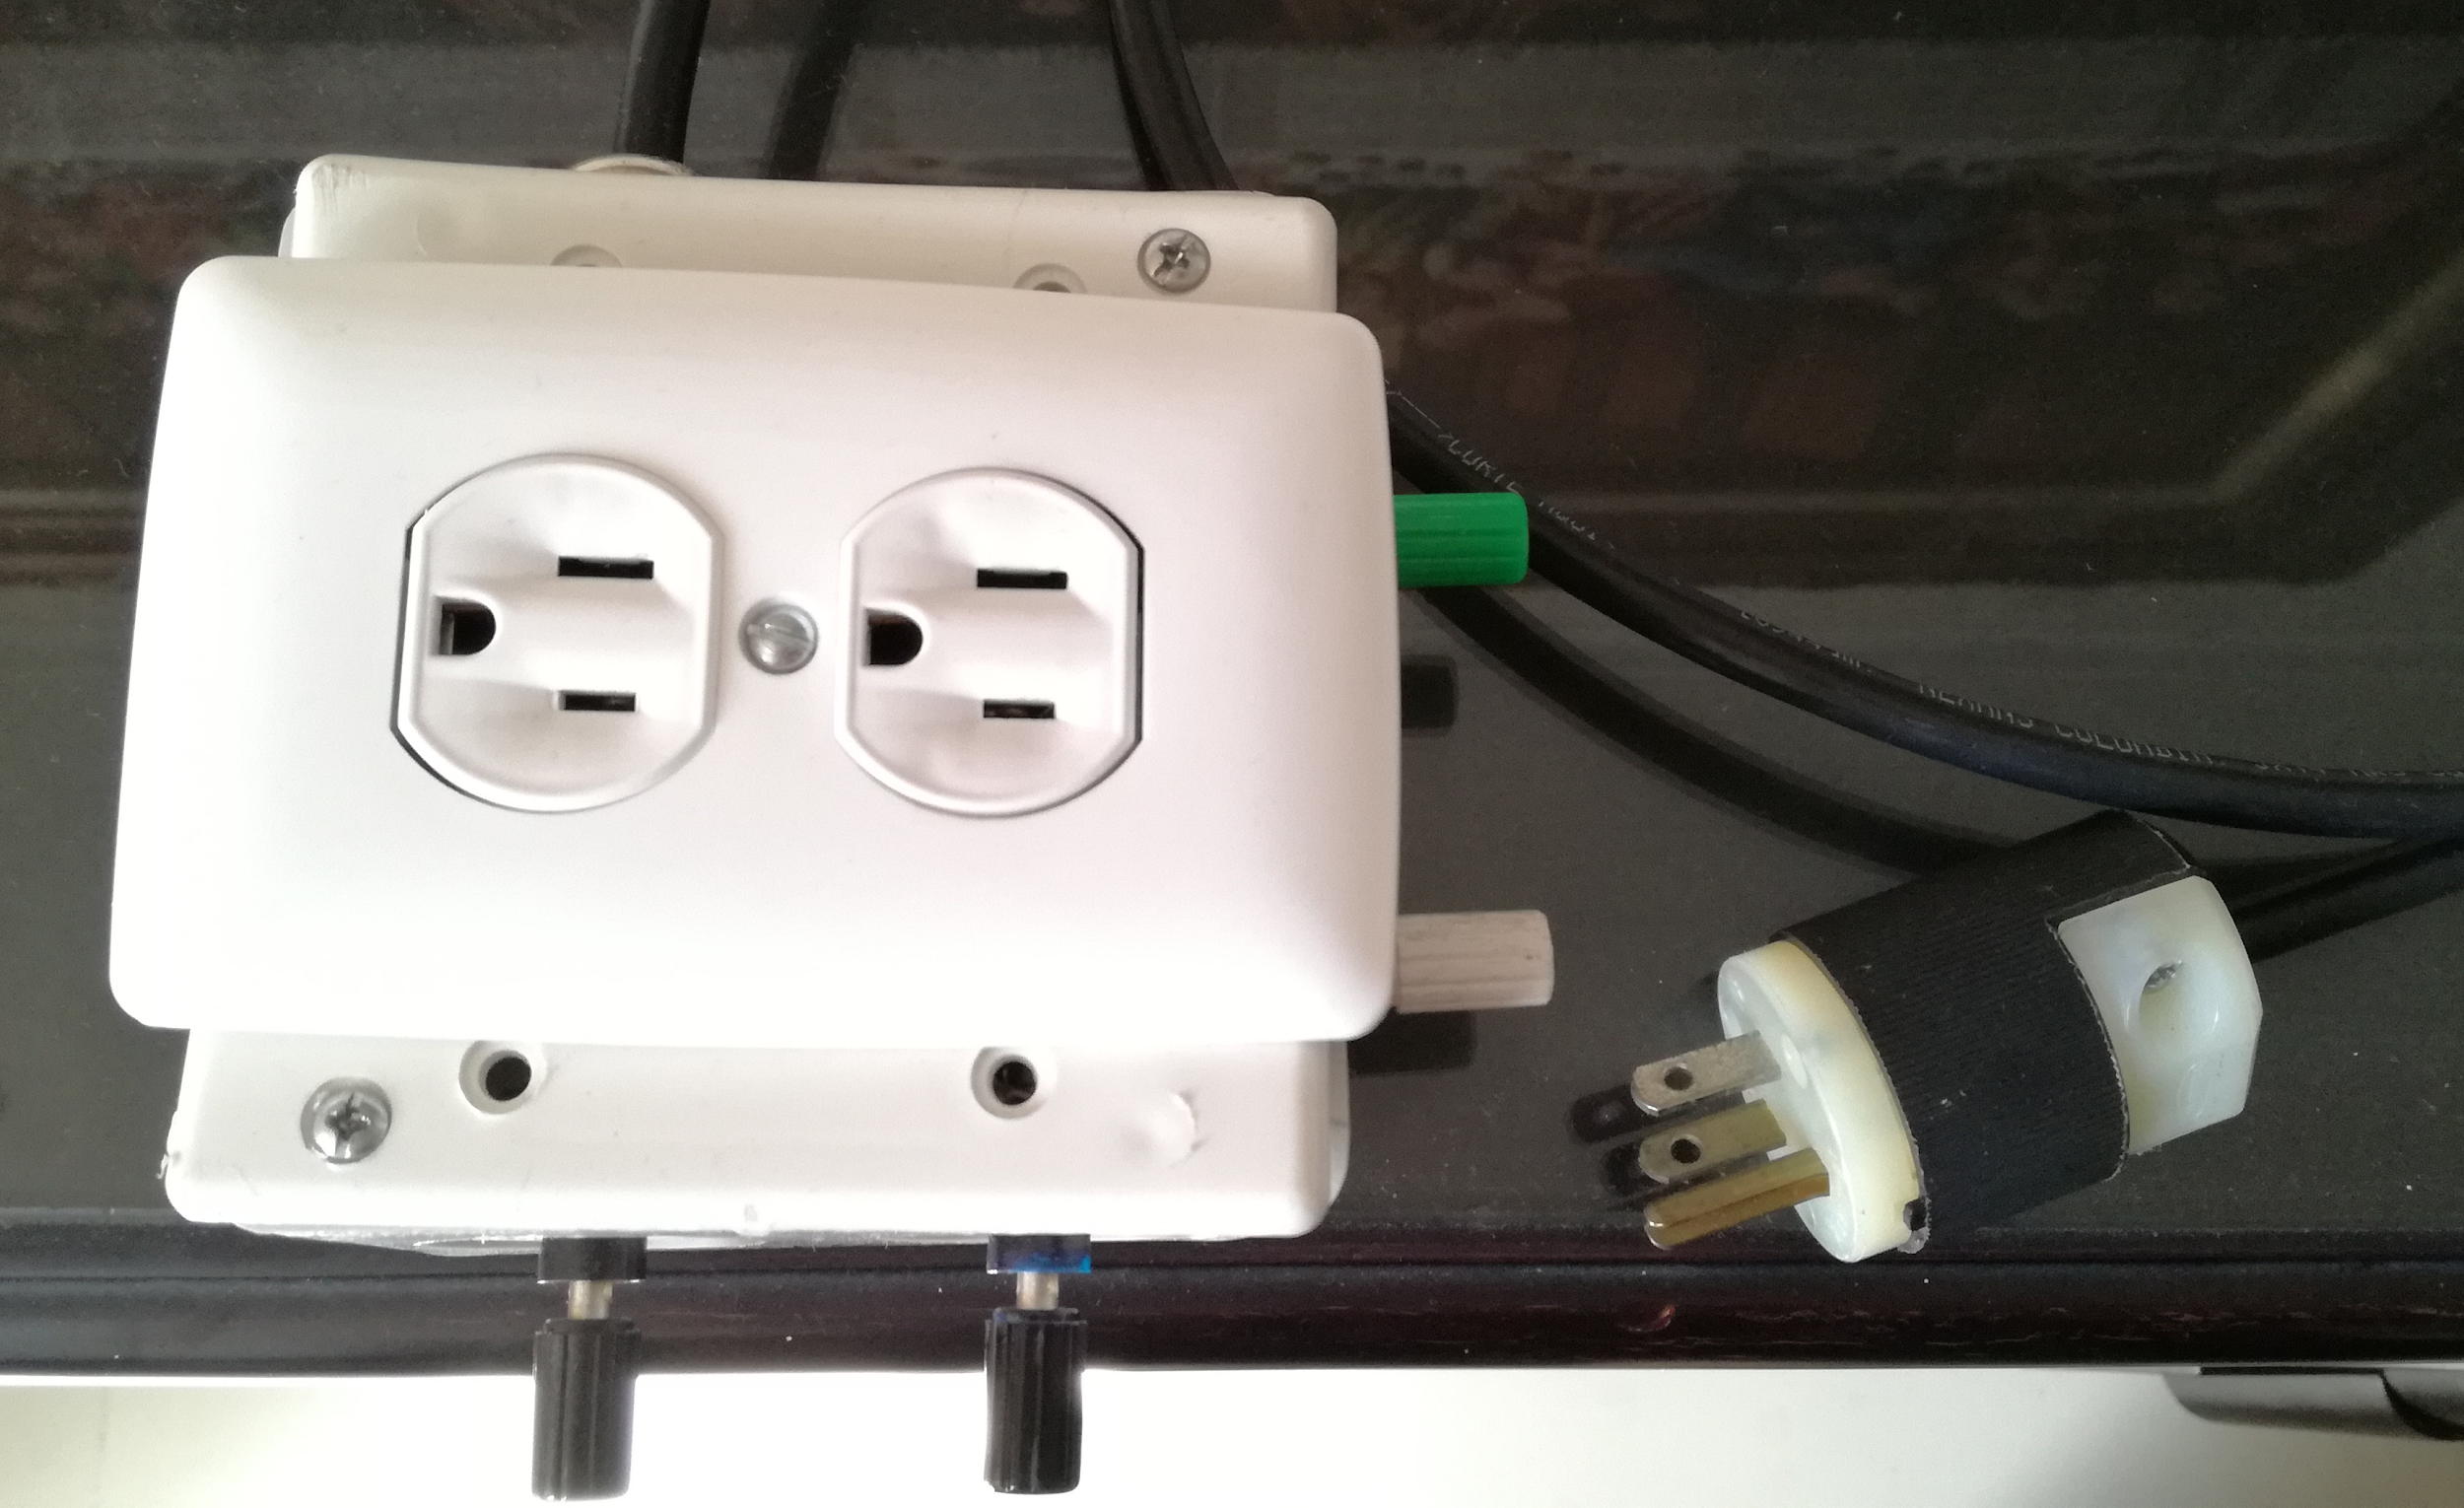
\includegraphics[clip,width=\columnwidth]{circuit_box.png}
\caption{Imagen del montaje del circuito.}
\label{circuit_box}
\end{figure}

En esta práctica se utilizaron tres cargas diferentes 
para analizar las formas de onda de corriente y tensión: 
Un \textit{cautin} como ejemplo de una carga puramente 
resistiva, un \textit{taladro} como carga inductiva y un 
\textit{computador portátil} como carga no lineal. 
Gracias a la inercia de la red eléctrica, la onda de 
tensión no depende de la carga, esto hace que la medida de 
la tensión sea similar para todas las cargas. Sin embargo, 
la onda de corriente depende de la impedancia de la carga. 
Por esta razón, el analisis de potencia se centrará 
en la forma de onda de la corriente, y se espera que 
la distorsión en la onda de tensión sea mínima. En otras 
palabras, mientras el valor de la Distorsión Total Armónica
de Tensión \textit{THD\textsubscript{V}} se mantenga más o
menos constante, el valor de la Distorsión Total Armónica
de Corriente \textit{THD\textsubscript{I}} varíe segun 
la carga que se esté midiendo.  \\

%For this practice three different loads are chosen to 
%analize their voltage and current waveform: 
%a soldering iron 
%like resistive load, a drill like inductive load and 
%a laptop like non-linear load. These loads are conected 
%to an electrical outlet, using the power meter. Owing to 
%high electrical network inertia, the voltage waveform do
%not depend on the load. For this reason, the voltage signal
%is similar in all measurings. However, current waveform 
%depend on impedance load and voltage, and the first 
%parameter is realted to load features. Therefore, the 
%power analysis will be centered on current waveform.\\

%\subsubsection{Solderin Iron (resistive load)}
%The current waveform is a pure sine signal and it does not 
%present any distortion and between voltage and current there
%are not phase difference. This can be observed in the Figure
%\ref{original_resistive_load}. 

\begin{figure}[h]
\centering
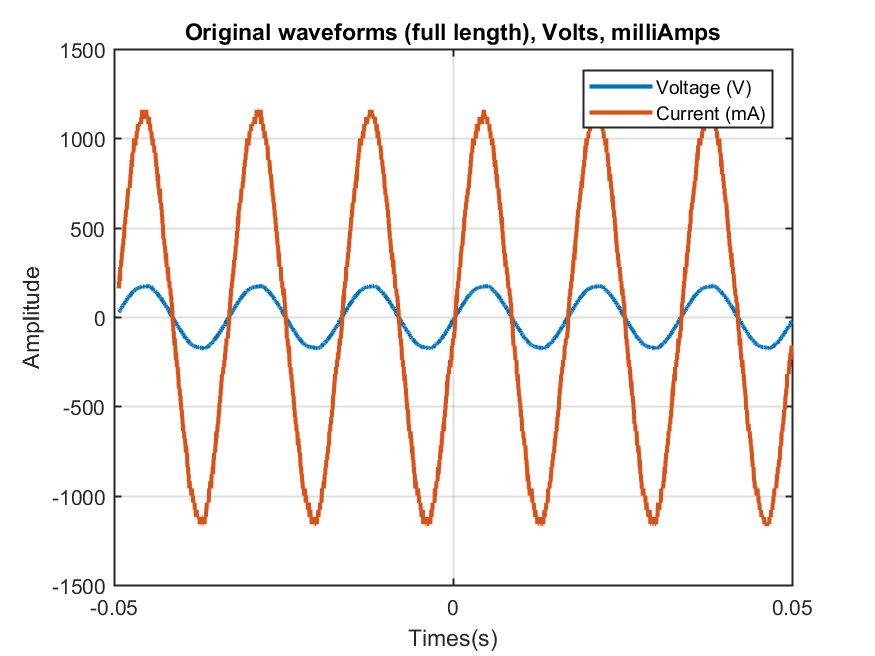
\includegraphics[clip,width=\columnwidth]{original_waveform_cautin.png}
\caption{Ondas de tensión y corriente para una carga
resistiva.}
\label{original_resistive_load}
\end{figure}

\subsubsection{Cautin (carga resistiva)}
La onda de corriente para esta carga fue una señal 
sinusoidal que no presentaba ninguna distorsión y además 
se encontraba en fase con la onda de voltaje. Las imágenes
de las formas de onda que se obtivieron en el osciloscopio 
se obseervan en la Figura \ref{original_resistive_load}. \\

%Additionally, in a resistive load, product between 
%current and voltage always 
%is positive, this means that soldering iron is a power 
%consumer and it is not able to supply energy. 

Adicionalmente, en una carga resistiva, el producto de la 
onda de corriente y tensión siempre es positivo, esto 
significa que un cautin funciona siempre como un 
consumidor de potencia ya que por su naturaleza no es 
capaz de entregar energía. \\

\begin{figure}[h]
\centering
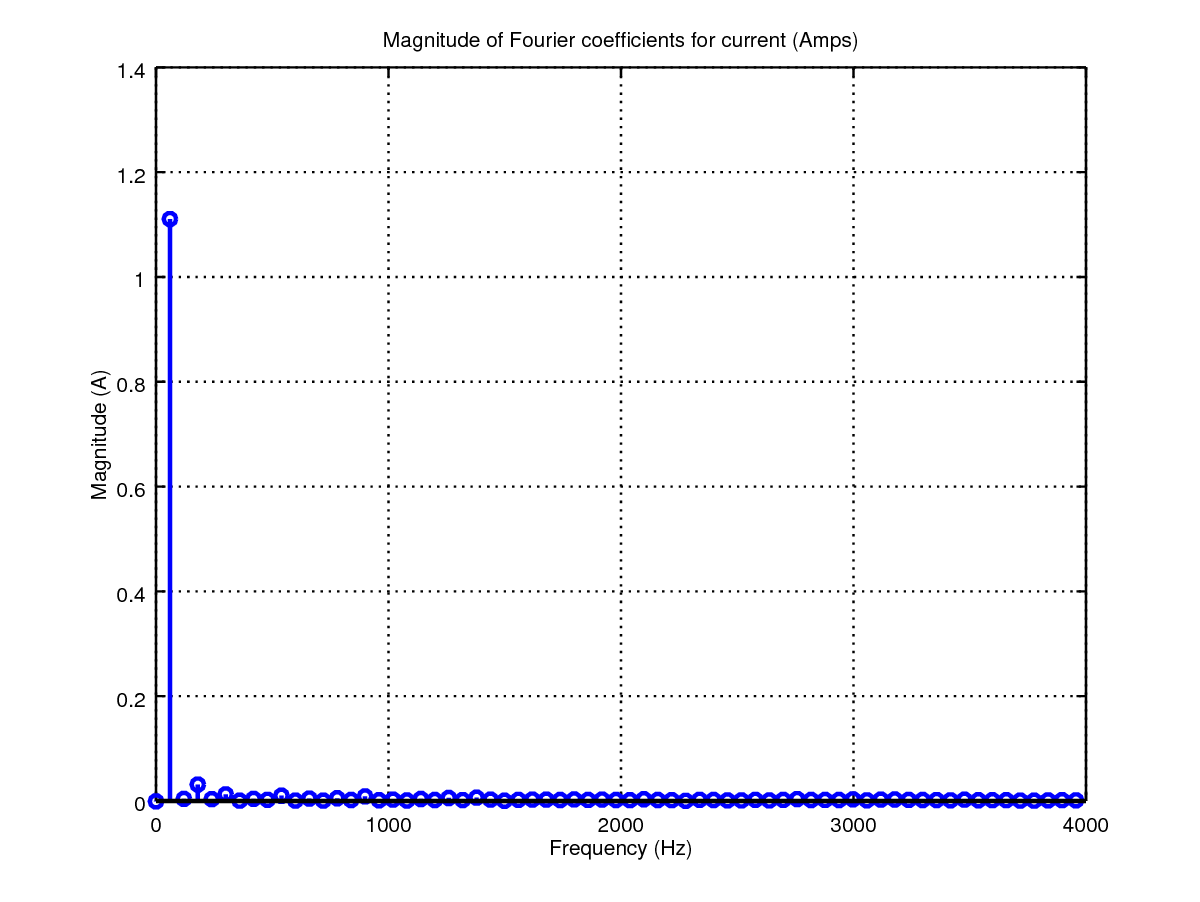
\includegraphics[clip,width=\columnwidth]
{zoomed_current_furier_coefficients_resistive.png}
\caption{Coeficientes de Fourier de la onda de corriente \\
para una carga resistiva.}
\label{fourier_corrent_coefficients_resistive}
\end{figure}

La Transformada de Fourier permite identificar las 
componentes armónicas de la señal de corriente. 
De acuerdo con la Figura 
\ref{fourier_corrent_coefficients_resistive}, la onda 
de corriente solamente tiene la componente de la frecuencia 
fundamental (60Hz), las demás son despresiables. 
Por tanto, no hay distorsión, el factor de potencia 
\textit{PF} es casi unitario, mientras que la Distorsión 
Total Armónica de Corriente 
\textit{THD\textsubscript{I}} es muy pequeña. Esto lo 
confirma la Salida 1, en donde el Factor de Potencia es 
0.9989, la potencia activa \textit{P} es muy alta en 
comparación a la potencia reactiva \textit{Q} y a la 
potenicia de distorsión \textit{D} 
y la Distorsión Armónica de Corriente 
\textit{THD\textsubscript{I}} es 4\%. 

%Fourier Transform allow to identify harmonic components of
%current signal. According to Figure
%\ref{fourier_corrent_coefficients_resistive}, current 
%waveform of a resistive load only have a 60 Hz component
%and it does not have any different harmonic component. So, 
%there are not distortion, the power factor \textit{PF} is 
%high and Total Harmonic Distortion \textit{THD} is 
%very small.
%This is an important feature from resistive loads.  

\begin{lstlisting}[caption = Carga resistiva.]
T     =     0.0167 s 
f0    =    59.9520 Hz 
Vrms  =   123.3322 V
Irms  =     0.7860 A
S     =    96.9336 VA
Pavg  =    96.8309 W 
P     =    96.8309 W 
Q     =    -1.8282 VAR 
D_fast=     4.0701 VA 
D     =     4.0562 VA 
PF    =     0.9989 
THD_V =     1.8878 %
THD_I =     4.0154 %
\end{lstlisting}

\subsubsection{Taladro (carga inductiva)}

\begin{figure}[h]
\centering
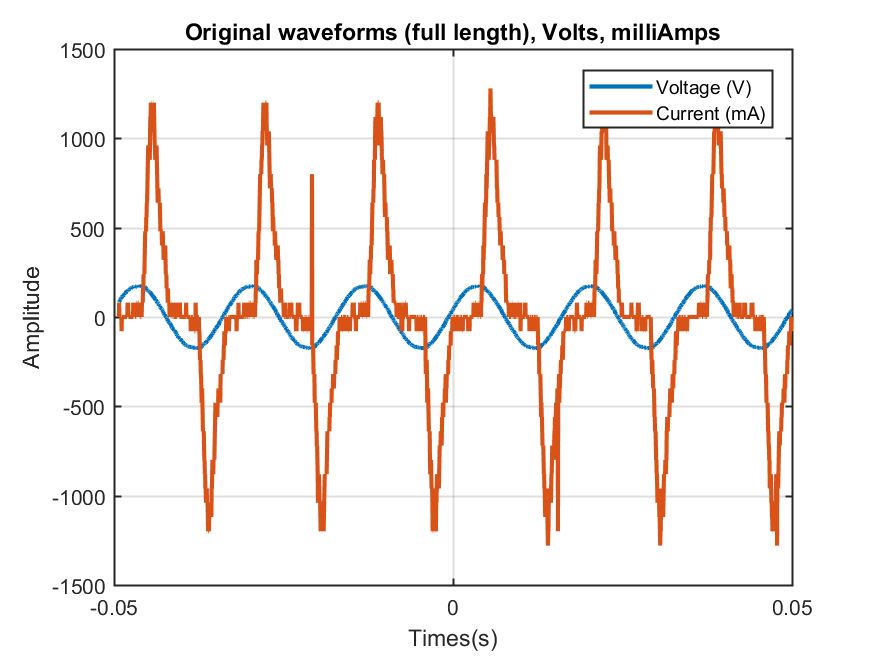
\includegraphics[clip,width=\columnwidth]
{original_waveform_drill.png}
\caption{Ondas de tensión y corriente para una carga
inductiva.}
\label{original_inductive_load}
\end{figure}

El comportamiento de la corriente en una carga inductiva 
es diferente al ocmportamiento en una carga resistiva. 
La forma de la corriente no es una puramente sinusoidal,
aparecen compoenentes armónicas que distorsionan la forma 
de la señal. La forma de onda de la corriente
se puede observar en la Figura 
\ref{original_inductive_load}.\\ 

\begin{figure}[h]
\centering
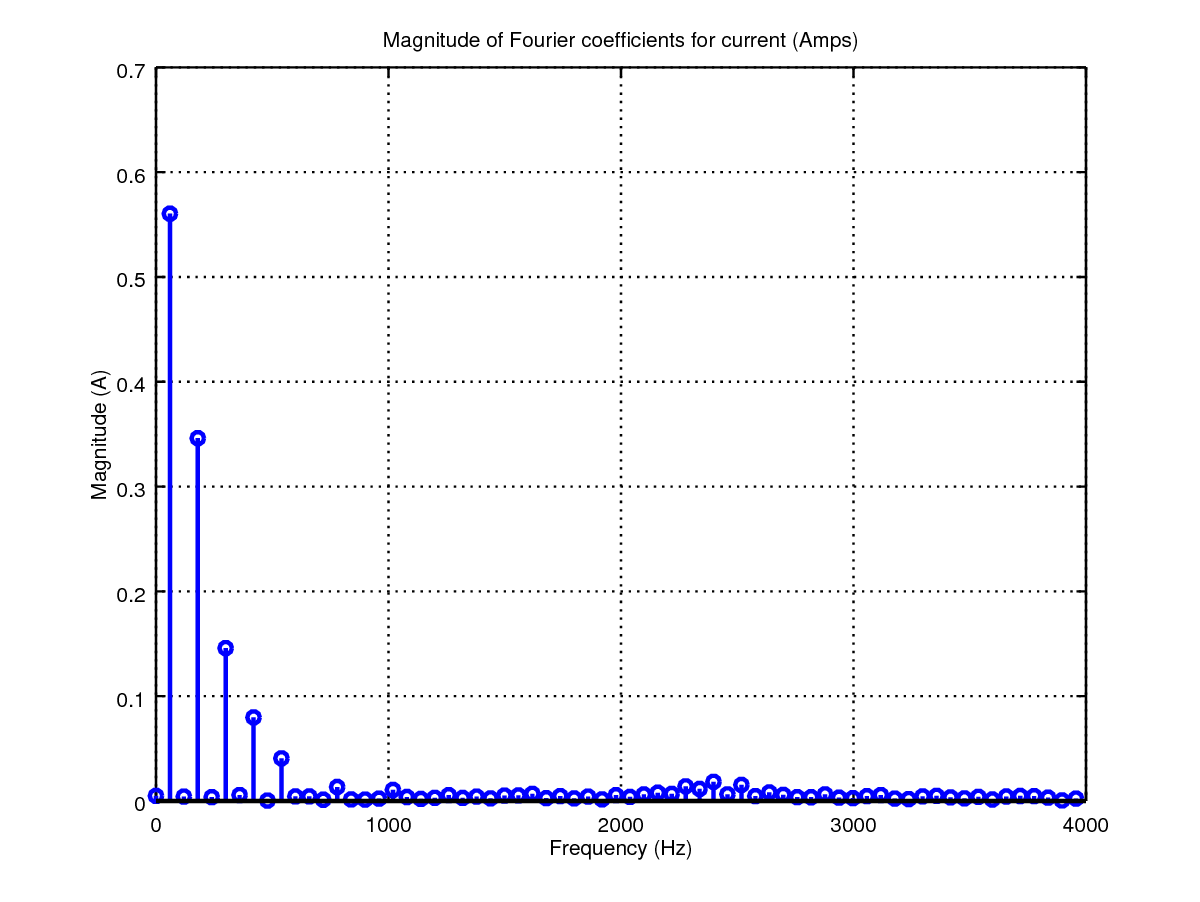
\includegraphics[clip,width=\columnwidth]
{zoomed_current_furier_coefficients_drill.png}
\caption{Coeficientes de Fourier de la  
onda de corriente \\ para una carga inductiva.}
\label{fourier_corrent_coefficients_inductive}
\end{figure}

La presencia de las componentes armónicas se observa 
con mayor claridad gracias a la Transformada de Fourier, 
esta transformada aparece en la Figura 
\ref{fourier_corrent_coefficients_inductive}.
La Transformada de Fourier de la señal de corriente 
presenta fuertes componentes armónicas en las frecuencias
$3 f_0$, $5 f_0$, $7 f_0$  y $9 f_0$, donde $f_0$ es la 
frecuencia fundamental (60Hz). Además de las componentes 
armónicas existe un desfase entre la onda de corriente 
y tensión. Este desfase es una característica importante 
de las cargas inductivas. \\

%\subsubsection{Drill (inductive load)} The current 
%behaviour for inductive loads is different to resistive 
%loads. Current waveform is not a pure sine signal, 
%because there are harmonic components that change shape 
%current signal. This can be observed in the Figure 
%\ref{original_inductive_load} and 
%\ref{fourier_corrent_coefficients_inductive}. 
%The waveform present peaks as a result of 
%current harmonic component: $3 f_0$, $5 f_0$, $7 f_0$ 
%and $9 f_0$,  where $f_0$ is fundamental frquency (60 Hz). 
%In addition, there are an 
%phase difference betweent both signal: current signal is
%slow respect to voltage signal.

A diferencia de una carga resistiva, la mediciones y 
los cálculos de potenicia en un taladro dieron como 
resultado un valor de  
Potencia Reactiva $Q$ y de Distorsión Total Armónica 
de Corriente mucho más alto. Tanto así que hacen 
que el valor del Factor de Potencia $pf$ sea muy bajo, 
aproximadamente 0.51. Los motores y otras cargas 
inductivas, por lo general tienen un factor de potencia 
más alto (entre 0.75 y 0.9), una causa por la cual el 
factor de potencia durante la medición fue mucho más 
bajo que estos valores es la presencia de un circuito 
eléctrico que regula la velocidad y el torque del 
motor del taladro. Este circuito electrónico para 
valores bajos de velocidad, genera distorsión en la 
señal de corriente la cual tiene el efecto de  
aumentar el \textit{THD\textsubscript{I}} y la Potencia 
de Distorsión $D$ y por tanto, reducir el Factor de 
Potencia. En la segunda parte de este informe se analizará
más detallamente el efecto de circuitos eléctronicos 
controladores de potencia. \\

\begin{lstlisting} [caption = {Output for inductive load.}
\label{output_inductive}]
T     =     0.0167 s 
f0    =    59.9520 Hz 
Vrms  =   123.8850 V
Irms  =     0.4831 A
S     =    59.8537 VA
Pavg  =    30.4372 W 
P     =    30.4372 W 
Q     =    38.7767 VAR 
D_fast=    33.9472 VA 
D     =    33.9434 VA 
PF    =     0.5085 
THD_V =     1.8561 %
THD_I =    69.7550 %
\end{lstlisting}

\subsubsection{Computador portátil (carga no-lineal)} 
Finalmente,  la forma de onda de la corriente y de la 
tensión se ilustran en la Figura 
\ref{original_no_lineal_load}. Se observa, en primer lugar
la presencia de picos bastante estrechos en la onda  
de corriente, esta forma de consumir 
es típica de muchos dispositivos electrónicos. 
La distorsión de la onda de corriente es tan alta que ya 
no es posible identificar una forma sinusoidal. 
Lo estrecho de los picos da una idea de la presencia de 
componentes armónicas con valores bastante altos. 

%according to Figure \ref{original_no_lineal_load},  
%current signal of non-linear load do not present any 
%sine shape. The current waveform present peaks more 
%narrow that inductive peaks loads. Those peaks 
%presents a high harmonic components which can be observed 
%in the Figure \ref{fourier_corrent_coefficients_nonlinear}. 
%The harmonic components of non-linear load are much higher 
%than harmonic components of inductive load. 

\begin{figure}[h]
\centering
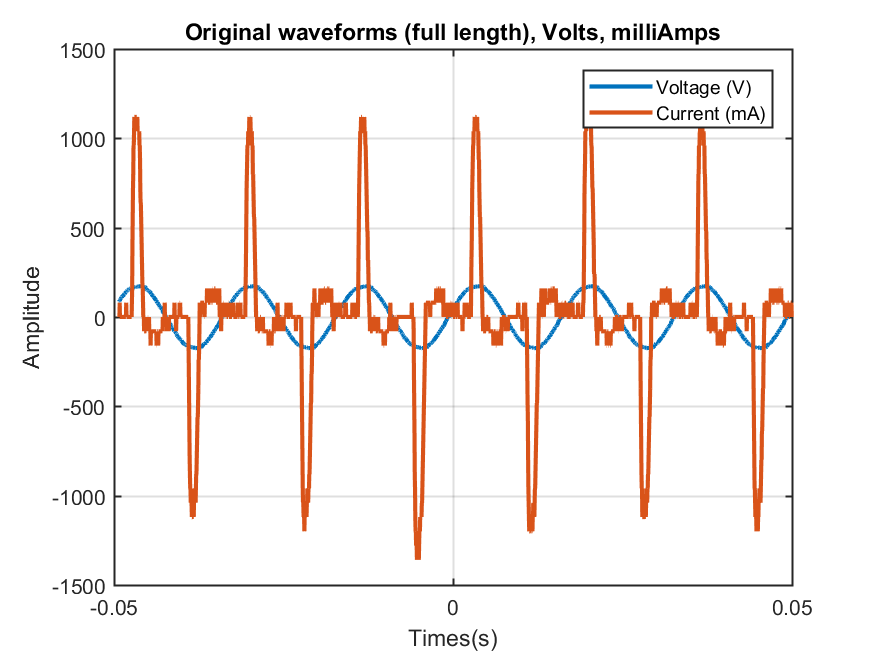
\includegraphics[clip,width=\columnwidth]
{original_waveform_computer.png}
\caption{Ondas de tensión y corriente para una carga
no-lineal.}
\label{original_no_lineal_load}
\end{figure}

Si se aplica la Trasformada de Fourier a la señal de 
corriente, se obtiene la Figura 
\ref{fourier_corrent_coefficients_nonlinear}. Se observa
que la magnitud de la segunda compoenente de frecuencia 
es mayor que la componente de la frecuencia fundamental. 
Y las compoenentes armónicas siguientes 
también tienen un valor bastante alto. 

\begin{figure}[h]
\centering
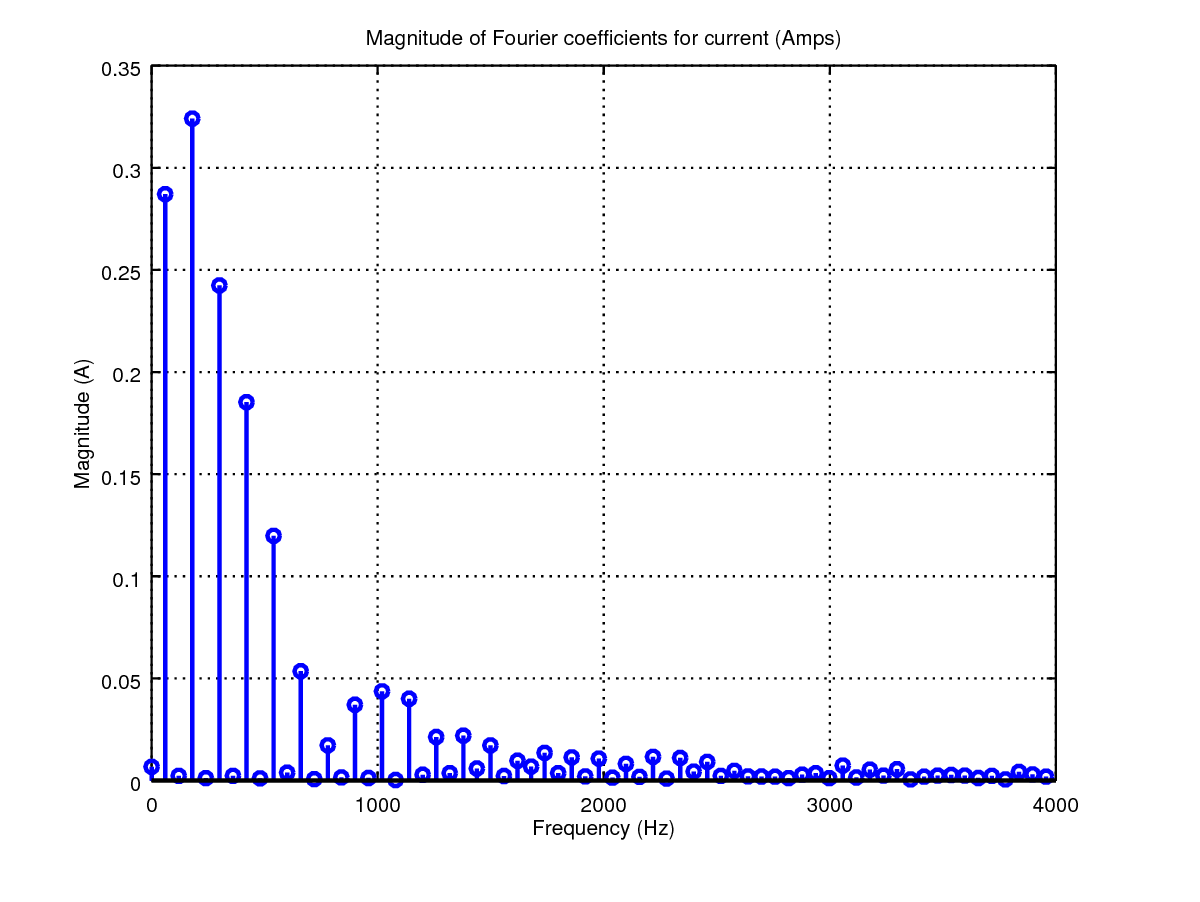
\includegraphics[clip,width=\columnwidth]
{zoomed_current_furier_coefficients_computer.png}
\caption{Coeficientes de Fourier de la onda de corriente\\
para una carga no-lineal.}
\label{fourier_corrent_coefficients_nonlinear}
\end{figure}

%Nevertheless, a laptop does not have reactives elements 
%like elctrical coils, the power factor values is very 
%low. The electronics circuits inside a laptop (or other 
%complex electronic device) do not respond linear way. 
%For this reason, current waveform presents a lot of 
%distortion, as a result, Harmonic Power $D$ and $THD_I$ 
%value are very high while $PF$ is small. 
A pesar que el computador portátil no posee grandes 
elementos rectivos, en comparación al motor de un taladro, 
el Factor de Potencia que se obtuvo fue muy bajo. 
Esto se debe a que los circuitos electrónicos no presentan
un comportamiento lineal en el consumo de la corriente.
El comportamiento no-lineal de este tipo de dispositivos 
es la causa de la alta distorisión de la onda de corriente, 
como resultado, el valor del Factor de Potencia \textit{pf}
es bajo, mientras que los valores de la 
Potencia de Distorsión $D$ y de
la Distorsión Total Armónica de Corriente son muy altos. 
En la Salida 3, pueden observarse los valores del Factor 
de Potencia, Potencia Activa $P$ y Potencia de 
Distorsión $D$ y Distorsión Total Armónica de Corriente 
y Tensión. 

\begin{lstlisting} [caption = Output for non-linear load.]
T     =     0.0167 s 
f0    =    59.9520 Hz 
Vrms  =   124.3447 V
Irms  =     0.3916 A
S     =    48.6915 VA
Pavg  =    23.9965 W 
P     =    23.9965 W 
Q     =    -5.7979 VAR 
D_fast=    41.9692 VA 
D     =    41.9644 VA 
PF    =     0.4928 
THD_V =     2.2668 %
THD_I =   164.9239 %
\end{lstlisting}

\subsection{Controlador AC}

Para la segunda parte de esta práctica, se diseñó un 
circuito usando tiristores para controlar la cantidad 
de potencia consumida por un bombillo. La intensidad 
de la luz del bombillo es controlada por medio de un 
potenciómetro. El circuito que se utilizó se muestra 
en la Figura \ref{ACcontroller}. 

%For the second part of the practice, a 
%circuit using thyristors  was desinged to control 
%the amount of power delivered to the light bulb. 
%The input is the 120 V AC and 
%the output is an AC waveform where there is a delay angle 
%before triggering the AC voltage. The phase control is 
%done with a potentiometer. The circuit designed is shown 
%in the Figure \ref{ACcontroller}.

\begin{figure}[h]
\centering
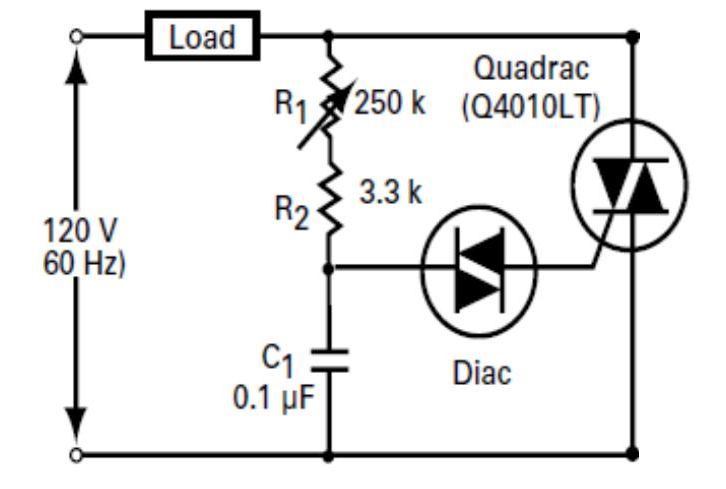
\includegraphics[clip,width=\columnwidth]{controller.png}
\caption{Circuito del controlador AC.}
\label{ACcontroller}
\end{figure}

Cuando el voltaje a través del capacitor alcanza el 
voltaje de ruptura del DIAC, éste se encuentra 
parcialmente descargado por el DIAC a través de la 
compuerta del QUADRAC. En ese momento el QUADRAC 
entra en modo conducción en el ciclo de media onda. 
En este circuito el QUADRAC se encuentra en los 
cuadrantes I y III. La simplicidad de este circuito 
hace que sea accesible para aplicaciones con pequeño 
control de rango. Los circuitos dimmer se basan en el 
control de potencia que se logra variando el ángulo de 
conducción del QUADRAC, de 30$^{\circ}$ a 160$^{\circ}$ 
cuando fluye la 
corriente por un potenciómetro que tiene la función de 
controlarla. \\

\begin{table}[h]
\begin{tabular}{|p{1.2cm}|c|c|c|c|c|c|}
\hline 
 & P  & Q  & D  & S  & PF & THDI  \\
 &(W) & (VAR) &(VA) & (VA) &  & (\%) \\ \hline  
NoCtrl & 77.24 & -3 & 3 & 77.36 & 0.999 & 4.01 \\ 
\hline 
Pos 0 & 74.2 & 0.1 & 5.1 & 74.37 & 0.998 & 6.23 \\ 
\hline 
Pos 1 & 69.8 & 10.5 & 17.29 & 72.68 & 0.96 & 23.99 \\
\hline 
Pos 2 & 53.64 & 23.48 & 31.41 & 66.45 & 0.807 & 53.48 \\
\hline 
Pos 3 & 40.19 & 27.81 & 35.69 & 60.51 & 0.664 & 73.58 \\ 
\hline
Pos 4 & 30.47 & 28.41 & 37.36 & 55.96 & 0.545 & 89.63 \\ 
\hline 
\end{tabular}
\caption{Mediciones de potencia para diferentes \\ valores 
del Potenciómetro.}
\end{table}

\section{CONCLUSIONES}

La carga resistiva muestra un factor de potencia de 
casi unitario. La carga inductiva tiene una forma de 
corriente rizada gracias al tipo de motor que se 
utiliza en el taladro. La carga no lineal muestra 
una forma de onda rizada que depende del circuito 
dentro del dispositivo electrónico. \\

El dimmer permite regular la potencia de la bombilla. 
Teniendo en cuenta que una bombilla es resistiva, la 
efectividad depende del voltaje y la corriente que se 
encuentra en éste. \\

El circuito controla la alimentación de la bombilla 
encendiendo y apagando durante las regiones positiva y 
negativa de la señal sinusoidal de entrada. Durante 
la parte negativa de la señal de entrada, se obtendrá 
el mismo tipo de respuesta, ya que tanto el DIAC como 
el QUADRAC se pueden disparar en la dirección inversa. 
Al variar la resistencia R, es posible controlar el
ángulo de conducción.\\

Acerca de las cargas inductivas y no lineales, no se 
debe utilizar el circuito dimmer, ya que ambos dependen 
del factor de potencia y de la forma de onda de tensión 
y corriente. \\

Los dispositivos electrónicos, como el DIAC y el QUADRAC, 
permiten construir circuitos para controlar la potencia 
de una carga resistiva.

\begin{thebibliography}{1}

\bibitem{IEEEhowto:kopka}
H.~Kopka and P.~W. Daly, \emph{A Guide to {\LaTeX}}, 3rd~ed.\hskip 1em plus
  0.5em minus 0.4em\relax Harlow, England: Addison-Wesley, 1999.

\end{thebibliography}

\end{document}